\subsection{Block-Diagonal Structure of Density Matrices}\label{sec:block-diagonal-structure}
\valert{
The fact that the spin representation $\mathcal{S}$ and the Majorana representation $\mathcal{M}$ are identical implies that the reduced density matrix might be of a block-diagonal form, in which the blocks are all identical. In this section, we discuss those operators that block-diagonalize the density matrix and elucidate their relation with the emergent gauge field. 
%
%However, this is only a hypothesis instead of a direct and rigorous proof of the existence of such a structure. 
%
%To see that the density matrix indeed has such a block-diagonal structure, we have to find the operator corresponding to each block that commutes with the density matrix. They are expected to be related to the emergent gauge fields, given that they give the gauge contribution of the entanglement.

%In addition, to make every block identical, there must be operators that provide equivalence relations among blocks.
}

In light of the physical pictures given by \cite{Yao-Qi_2010} and \cite{Xu-Rakovszky-Knap-Pollmann_2025}, the operators that block-diagonalize the density matrix are defined at the boundary of the subregion because the block-diagonal structure of the reduced density matrix is due to the Gauss law of the gauge field~\cite{Xu-Rakovszky-Knap-Pollmann_2025}. Suppose the Gauss law in a gauge theory defined on a lattice is $\sum_{j\in \mathcal{N}_i}E_{ij} = \rho_i$, where $\rho_i$ is the matter field on the lattice site $i$, $E_{ij}$ is the electric field residing on the edge $\anglelr{ij}$, and $\mathcal{N}_i$ is the set of nearest neighbors of the site $i$. The boundary of the chosen subregion \textit{splits} the Gauss law of some neighborhoods $\mathcal{N}_i$ that cross the boundary, causing entanglement between the subregion and the environment because the Gauss law relates the matter field outside the subregion with the gauge field at the boundary, which is partly inside the subregion. Each \textit{residue} Gauss law at the boundary then acts as a symmetry operator that block-diagonalizes the reduced density matrix. 

In the Kitaev model, a problem is that the Gauss law of the gauge theory, which reads $b^x_ib^y_ib^z_ic_i = \mathds{1}$, only exists in the Majorana representation. Another issue is that the fundamental degrees of freedom of the Kitaev model reside on the lattice sites of the lattice, but the electric field operators $E_{ij}$ of the gauge theory, defined by $\mrm{e}^{i E_{ij}} = b^{\alpha_{ij}}_i$, live on edges, and which are not well-defined in the original setting of the model. For these reasons, we cannot directly apply the method proposed by~\cite{Xu-Rakovszky-Knap-Pollmann_2025}. %Some modifications are necessary.

Our solution to this issue is to transform a Majorana fermion theory coupled to a gauge field back to the physical spin representation by \textit{gluing} pairs of fermions using string operators. 
%As we have noted earlier, the residual electric field inside the subregion after tracing out the environment is proportional to the exponent of $b$-Majorana fermions at the boundary, with the direction pointing outward. 
Suppose there are an even number $\abs{\de A} = 2L$ of edges that cross the boundary of the simply-connected region $A$. The corresponding set of $b$-Majorana fermions encoding the residual electric field is $\lrg{b^{\mu_1}_{i_1}, b^{\mu_2}_{i_2}, b^{\mu_3}_{i_3},\cdots,b^{\mu_{2L}}_{i_{2L}}}$, where $\mu_k$ represents the direction of the $k$-th edge crossing the boundary, which is connected to site $i_k$. 
To transform these $b$-Majorana fermions to a physical representation, we insert gauge-field operators along strings $\mathcal{C}_1, \mathcal{C}_2, \mathcal{C}_3,\cdots, \mathcal{C}_{L}$ that link pairs of Majorana fermions $(b^{\mu_1}_{i_1},b^{\mu_2}_{i_2}), (b^{\mu_3}_{i_3},b^{\mu_4}_{i_4}),\cdots,(b^{\mu_{2L-1}}_{i_{2L-1}},b^{\mu_{2L}}_{i_{2L}})$, respectively, to create a series of physical operators of the form
\begin{equation}\label{equ.b-link}
    b^{\mu_{2n-1}}_{i_{2n-1}} \lr{\prod_{\anglelr{ij}\in\mathcal{C}_{n}} \hat{u}_{ij}}b^{\mu_{2n}}_{i_{2n}} \quad ; \quad n=1,2,3,\cdots, L
\end{equation}
in which the two $b$-Majorana fermions $b^{\mu_{2n-1}}_{i_{2n-1}}$ and $b^{\mu_{2n}}_{i_{2n}}$ are at the endpoints of the string $\mathcal{C}_n$, and the product of gauge-field operators in between is the string that links the two endpoints together. 
\begin{figure}
    \centering
    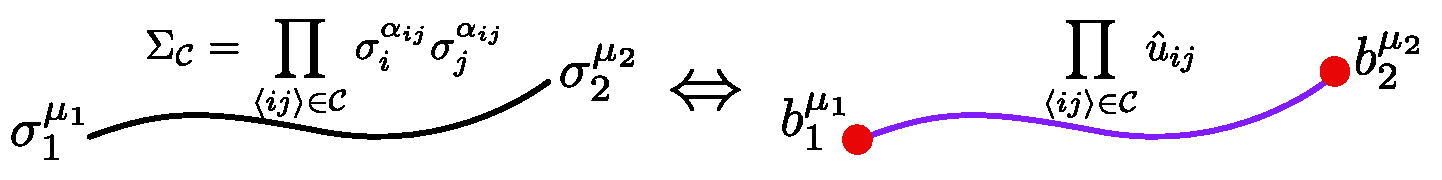
\includegraphics[width=\linewidth]{figures/linking-string-electric-field.pdf}
    \caption{Two $b$-Majorana fermions can also be linked by a series of gauge-field operators, $\prod_{\anglelr{ij}\in\mathcal{C}} \hat{u}_{ij}$. In that way, a physical operator $\hat{\xi}$ is constructed.}
    \label{fig.linking-strings-electric-field}
\end{figure}
However, the expression \eqref{equ.b-link} only contains $b$-Majorana fermions and cannot be transformed directly to the spin representation. To obtain physical strings containing purely spin operators, we can further insert $c$-Majorana fermions into the expression \eqref{equ.b-link}, then we obtain the following result   
\begin{equation}\label{equ.c-b-link}
    b^{\mu_{2n-1}}_{i_{2n-1}}c_{i_{2n-1}} \lr{\prod_{\anglelr{ij}\in\mathcal{C}_{n}} c_i\hat{u}_{ij}c_j}c_{i_{2n}}b^{\mu_{2n}}_{i_{2n}}.
\end{equation}
%in which those inserted $c$-Majorana fermions are identities $cc=\mathds{1}$, thus everything remains the same. 
%
After considering the transformation $\sigma^\mu_i\to ib^\mu_ic_i$, the operator \eqref{equ.c-b-link} is equal to the operators $\hat{\xi}_n$ defined in the following way
\begin{equation}\label{equ.spin-string-linking-gauge}
    \hat{\xi}_n \equiv \sigma^{\mu_{2n-1}}_{i_{2n-1}}\Sigma_{\mathcal{C}_n}\sigma^{\mu_{2n}}_{i_{2n}} \quad ; \quad n=1,2,3,\cdots ,L
\end{equation}
up to a phase that depends on the lengths of the strings $\abs{\mathcal{C}_n}$. The process of producing $\hat{\xi}$-operators from \eqref{equ.b-link} to \eqref{equ.spin-string-linking-gauge} is illustrated in \autoref{fig.linking-strings-electric-field}. All $\hat{\xi}_n$ operators defined in a simply-connected subregion $A$ commute with the reduced density matrix $\rho_A$. 
\begin{figure}
    \centering
    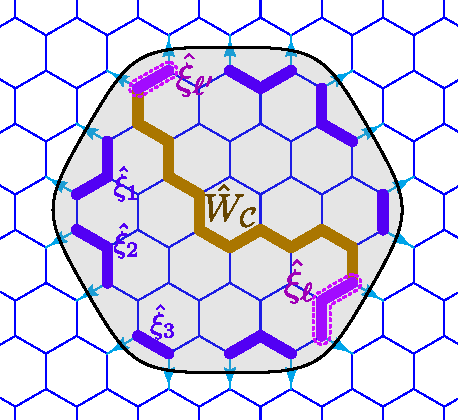
\includegraphics[width=0.8\linewidth]{figures/xi-wilson-flip.pdf}
    \caption{\alert{The electric-field operators living on the edges crossing the boundary of the region are split in half, as shown in the first panel. In the physical spin representation, these electric fields correspond to the spin operators $\sigma^\mu$ with directions pointing outwards. The second panel displays string operators that connect two adjacent spins in the first panel in a pair. Multiplying the first panel by the second one gives a series of operators $\hat{\xi}$, as shown in the third panel. Applying the same method but with the pairing order shifted yields another set of operators $\hat{\zeta}$, as showcased in the last panel.}}
    \label{fig.xi-def}
\end{figure}
The first three panels of \autoref{fig.xi-def} illustrate an example of the process of defining $\hat{\xi}$-operators using the method given by \eqref{equ.spin-string-linking-gauge}. 
%The directions of the spin operators at the endpoints of the links point outward, representing the gauge fields being cut. In the first panel are the spin operators $\sigma^\mu_i$, which are exactly the spin operators shown in equation \eqref{equ.spin-string-linking-gauge}, at the boundary with their directions pointing outwards. In the next panel, we subsequently multiply the string operators $\Sigma_{\mathcal{C}_n}$, which is the string operator shown in equation \eqref{equ.spin-string-linking-gauge} that lies between the two spin operators residing on the two endpoints of the string, with the spin operators set previously. After that, such operators are used as definitions of $\hat{\xi}_n$'s, which are illustrated in the third panel of \autoref{fig.xi-def}. In this example, we now focus on $\hat{\xi}_1$, which is defined as
%\[
%\hat{\xi}_1 = \sigma^y_1\lr{\sigma^x_1\sigma^x_2}\sigma^z_2 \propto \sigma_1^z\sigma_2^y.
%\]
%The subscript ``1'' indicates the lower-left endpoint of the dimer, while ``2'' stands for the other one. It can be shown that $\hat{\xi}_1$ commutes with every string operator $\Sigma_{\mathfrak{D}}$ with $\mathfrak{D}\subset A$ in a trivial way by examining all possible strings that reach the two endpoints of the dimer where $\hat{\xi}$ lives. By doing so, one will find that either (i) at one endpoint of a string $\mathcal{C}$, which is right at one of the two endpoints of the $\hat{\xi}_1$ dimer, is a spin operator whose direction is parallel to the spin operator of $\hat{\xi}_1$ on that endpoint; Or (ii) none of the two spin operators of $\Sigma_{\mathcal{C}}$, whose positions are the two endpoints of $\hat{\xi}_1$, is parallel to the spin operator of $\hat{\xi}_1$ at its position, such that the twice of sign flipping caused by the anti-commutation of Pauli algebra between $\Sigma_{\mathcal{C}}$ and $\hat{\xi}_1$ gets the positive sign again. 
%These situations, along with the fact that $[\hat{\xi}_1,W_p]=0\;\forall p$~\footnote{A loop also counts as a string, just with two endpoints at the same position, therefore, proving that every string operator commutes with $\hat{\xi}_n$ also proves that every plaquette operator commutes with $\hat{\xi}_n$ at the same time.}, 
By exhausting all possible string operators in the subregion and the commutation relations among spin operators, we prove that $[\hat{\xi}_n,\rho_A]=0\;\forall n$ because $\rho_A$ consists of string operators inside $A$. 
%In the same sense, we may generalize this statement to $[\hat{\xi}_n,\rho_A]=0\;\forall n$, where the operators $\hat{\xi}_n$ are defined through the process illustrated in \autoref{fig.xi-def} in $A$. 
At the same time, the regions where $\hat{\xi}$-operators are supported have no intersection, hence they commute with each other, $[\hat{\xi}_m,\hat{\xi}_n]=0\;\forall m,n$. Therefore, the set $\lrg{\xi_1,\cdots,\xi_L}$ of expectation values of $\hat{\xi}$-operators defined in $A$ forms good quantum numbers that block-diagonalizes the reduced density matrix $\rho_A$
\begin{equation}\label{equ.rho-block-diagonal-structure}
    \rho_A = \bigoplus_{\lrg{\xi_1,\cdots,\xi_L}} \varrho_{\lrg{\xi_1,\cdots,\xi_L}}
\end{equation}
where each $\varrho_{\lrg{\xi}}$ is the block labeled by a set of binaries $\lrg{\xi}$, and thus the number of blocks is $2^{L} = 2^{\abs{\de A}/2}$.

\alert{In defining $\hat{\xi}$-operators, the way we chose to pair points along the boundary was like $(b^{\mu_1}_{i_1},b^{\mu_2}_{i_2}), (b^{\mu_3}_{i_3},b^{\mu_4}_{i_4}),\cdots,(b^{\mu_{2L-1}}_{i_{2L-1}},b^{\mu_{2L}}_{i_{2L}})$. However, it is not the only way to pair these points. We can choose another way in which the pairing order is shifted by one compared to the previous way we adapted for $\hat{\xi}$-operators
\[
(b^{\mu_2}_{i_2},b^{\mu_3}_{i_3}), (b^{\mu_4}_{i_4},b^{\mu_5}_{i_5}),\cdots,(b^{\mu_{2L}}_{i_{2L}},b^{\mu_1}_{i_1})
\]
and then connect each of them through a new set of strings $\{\mathcal{C}'_n\}$. In this way, a set of operators $\hat{\zeta}_n$ can be defined
\begin{equation}\label{equ.spin-string-linking-gauge-zeta}
    \hat{\zeta}_n \equiv \sigma^{\mu_{2n}}_{i_{2n}}\Sigma_{\mathcal{C}'_n}\sigma^{\mu_{2n+1}}_{i_{2n+1}} \quad ; \quad n=1,2,3,\cdots, L
\end{equation}
where the periodic notational convention $i_{2L+1}=i_1$ and $\mu_{2L+1}=\mu_1$ is used. In the same sense, these $\hat{\zeta}$-operators also commute with the reduced density matrix. An example of a set of $\hat{\zeta}$-operators is illustrated in the fourth panel of \autoref{fig.xi-def}, from which we can see that the pattern of $\hat{\zeta}$-operators differs from that of $\hat{\xi}$-operators by shifting a unit along the boundary, so that each $\hat{\xi}_n$ is in between $\hat{\zeta}_{n-1}$ and $\hat{\zeta}_n$. According to the algebraic rules of Pauli matrices, a relation between $\hat{\xi}$-operators and $\hat{\zeta}$-operators can be obtained directly
\begin{equation}\label{equ.xi-zeta-relation}
    \hat{\zeta}_n\hat{\xi}_m\hat{\zeta}_{n} =
\left\{
\begin{array}{ll}
   -\hat{\xi}_m &;\; \text{for $m=n\vee n+1$} \\
   \hat{\xi}_m  &;\; \text{otherwise} 
\end{array}
\right.
\end{equation}
This equation implies that the $\hat{\zeta}$-operators relate different blocks of the density matrix $\rho_A$ in the way that
\begin{equation}\label{equ.related-blocks}
    \hat{\zeta}_n \varrho_{\lrg{\cdots,\xi_n,\xi_{n+1},\cdots}}\hat{\zeta}_n^\dagger = \varrho_{\lrg{\cdots,-\xi_n,-\xi_{n+1},\cdots}}
\end{equation}
By this relation, any two blocks $\varrho_{\lrg{\xi}}$ and $\varrho_{\lrg{\xi'}}$ in $\rho_A$ can be related, and thus their sets of eigenvalues are identical. However, a $\hat{\zeta}$-operator flips the eigenvalues of two $\hat{\xi}$-operators at the same time, so only two blocks with the same total parity $\prod_{i=1}^{L}\xi_i$ of the set $\lrg{\xi}$ are related by a specific set of $\hat{\zeta}$-operators.}



